\documentclass[a4paper,oneside,12pt]{article}

\usepackage[slovene]{babel}    % slovenian language and hyphenation
\usepackage[utf8]{inputenc}    % make čšž work on input
\usepackage[T1]{fontenc}       % make čšž work on output
\usepackage[reqno]{amsmath}    % basic ams math environments and symbols
\usepackage{amssymb,amsthm}    % ams symbols and theorems
\usepackage{url}               % \url and \href for links
\usepackage{icomma}            % make comma a thousands separator with correct spacing
\usepackage{graphicx}          % slike
\usepackage{enumitem}          % seznami
\usepackage[bookmarks, colorlinks=true, linkcolor=black, anchorcolor=black,
  citecolor=black, filecolor=black, menucolor=black, runcolor=black,
  urlcolor=black, pdfencoding=unicode]{hyperref}  % clickable references, pdf toc
\usepackage[
  paper=a4paper,
  top=2.5cm,
  bottom=2.5cm,
  left=2.5cm,
  right=2.5cm
% textheight=24cm,
% textwidtht=16cm,
]{geometry}  % page geomerty

\pagestyle{empty}              % vse strani prazne
\setlength{\parindent}{0pt}    % zamik vsakega odstavka
\setlength{\parskip}{10pt}     % prazen prostor po odstavku
\setlength{\overfullrule}{30pt}  % oznaci predlogo vrstico z veliko črnine

\usepackage{tabularx}

\begin{document}

\begin{minipage}[t]{0.7\linewidth}
Študentski svet Fakultete za matematiko in fiziko \\
Jadranska 19 \\
1000 Ljubljana \\

Ljubljana, \today\\
\end{minipage}%
\begin{minipage}[t]{0.3\linewidth}
  \mbox{} \\[-15pt]
  \hspace*{\fill} 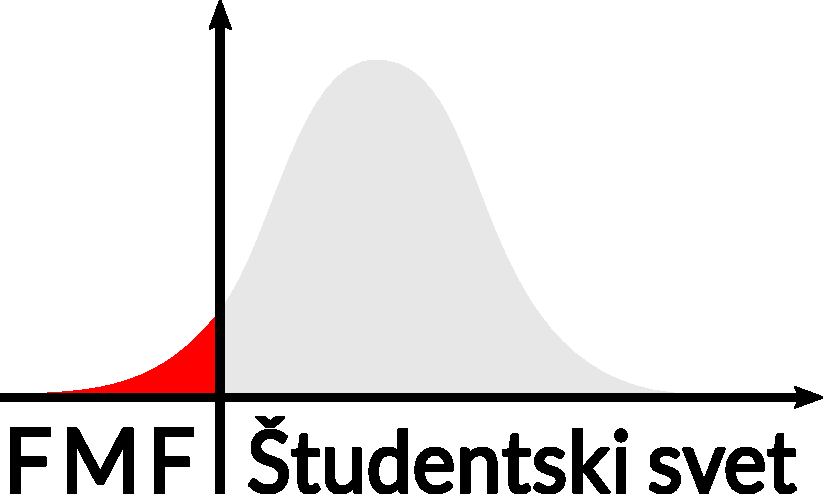
\includegraphics[width=0.9\linewidth]{ssfmf_logo_col.pdf}
\end{minipage}

\textbf{Obrazec za kandidaturo na volitvah v Študentski svet FMF v letu 2017/18} \\[-0.5ex]

Ime in priimek: \hrulefill \\[3ex]
Oddelek, smer in letnik: \hrulefill \\[3ex]
Elektronska pošta: \hrulefill \\[3ex]
Telefon: \hrulefill \\[3ex]
Datum: \hrulefill \hspace{1em} Podpis: \hrulefill \\[-2ex]

Kandidiram za naslednje funkcije (ustrezno obkroži): \\[1ex]
ČLAN ŠS \hfill
KOMISIJA ZA ŠTUDENTSKA MNENJA \hfill
SENAT \\[1ex]
UPRAVNI ODBOR \hfill
ZNANSTVENO PEDAGOŠKI SVET OM \\[1ex]
ZNANSTVENO PEDAGOŠKI SVET OF \hfill
AKADEMSKI ZBOR \\[1ex]
DISCIPLINSKA KOMISIJA \hfill
KOMISIJA ZA ETIČNA VPRAŠANJA \\[1ex]
KOMISIJA ZA KAKOVOST \hfill
KOMISIJA ZA SAMOEVALUACIJO

Seznam podpornikov:

\renewcommand{\arraystretch}{1.4}
\begin{tabularx}{\textwidth}{|XX|X|X|} \hline
 \multicolumn{2}{|l|}{\textbf{Ime in priimek}} & \textbf{Vpisna številka} & \textbf{Podpis} \\ \hline
  & & & \\ \hline
  & & & \\ \hline
  & & & \\ \hline
  & & & \\ \hline
  & & & \\ \hline
  & & & \\ \hline
  & & & \\ \hline
  & & & \\ \hline
  & & & \\ \hline
  & & & \\ \hline
\end{tabularx}

H kandidaturi priložite potrdilo o vpisu (lahko kopijo) in vse skupaj
oddajte v predal ŠS pri recepciji na Jadranski 19 (stavba fizike).

\end{document}
